
\documentclass{IEEEtran}

\usepackage{amsmath}
\usepackage{amssymb}
\usepackage{graphicx}
\usepackage{caption}
\usepackage{booktabs}
\usepackage{pdfpages}
\usepackage{hyperref}

\title{Modeling Uppsala Temperature \\ A Bayesian Approach}
\author{Shahab Sherveh}

\begin{document}
    \maketitle
    \begin{abstract}
      In this report we will explore the Uppsala temperature dataset and try to find a suitable Bayesian model for it to be able to provide a forecast for the future. To do so, the data is divided into training and test sets. The training set is used to fit and produce a posterior and evaluate the model using posterior predictive check and using ELPD(expected log point-wise density). And the test is used to evaluate the model performance in the future using CRPS(continuous ranked probability score). We will try two models one an AR(1)abbreviation for auto regressive with order 1 and another one which included an extra Seasonal component. And we conclude that the model with the seasonal component is better in terms of ELPD and CRPS. Our code is written in python using PyMC for MCMC implementation.
    \end{abstract}

    \section{Introduction}
    Modeling weather, particularly temperature, is crucial for a wide range of applications across science, industry, and daily life. For instance, the temperature forecast could be used to have an estimate on the crops productions \cite{Lobell_2007}. This wide range of applications necessitates the development of robust statistical models that can capture the underlying patterns. However, while it is important to be accurate as much as possible, it is also important to take into account the uncertainty of our modeling model or the data itself. On the other hand, We may also wish to incorporate assumptions about evident patterns or specific future scenarios.. This is where the Bayesian Modeling comes into play, in which we could easily add uncertainty by just increasing the variance of the prior distribution. Or we could in case of time-series we could add a trend or seasonal component to provide some already know information into the model or even assume a downward trend. While, this amount of flexibility is a great advantage compared to the frequentist approach, it comes with the price of computation complexity and convergence issues introduced by MCMC algorithm.

    Through the following sections, we will introduce the dataset and the preprocessing steps we took to prepare the data for the modeling. Then a short theoretical background on the state-space models and the structural auto regressive models are discussed. After that, the chosen models and their implementations are discussed then their performance is evaluated separately then compared to each other. And finally, we conclude the report with a summary of the findings and future works.

    \section{Dataset}
    The dataset we used is published and processed by Bergström \cite{BergstromHans2002Data} and is publicly available at Swedish Meteorological and Hydrological Institute (SMHI) \cite{SMHI}. The dataset contains daily mean temperature in Uppsala, Sweden from 1722 to 2022. It was recorded by hand until 1985 and published in bulletins. After that it was stored on computers. The data is homogenized and the missing values are handled by the publishers. The data is available in a txt format where each column is separated by spaces and the rows are separated by new lines. The columns are \textit{Year}, \textit{Month}, \textit{Day}, \textit{Mean Temperature} and \textit{Corrected Mean Temperature}. It is interesting to note that Erik Burman, professor of astronomy, initiated the observations in the 1720s. A young student, Anders Celsius – who later became professor of astronomy at the university and who invented the 'Celsius' or 'Centigrade' thermometer scale, was actually carrying out the observations, and was responsible for them after Burman’s death in 1728 \cite{BergstromHans2002Data}
    \subsection{Preprocessing}
    The data is clean enough to read into a pandas dataframe without much problem. and the columns are renamed to \textit{Year}, \textit{Month}, \textit{Day} , \textit{MeanTemperature} and \textit{CorrectedMeanTemperature} where \textit{CorrectedMeanTemperature} is used as our single observed variable. The data is then downsampled to monthly data by taking the average of the data points in each month to reduce the noise and the total number of data points. The total number of data points are 3612. The last 10 years ($12\times10=120$ points) is kept as test set with which the models performance are evaluated for the future performance. The rest of the data ($3612-120=3492$ points) is used as training set.

    \subsection{Exploratory Data Analysis}
    The data is plotted in figure \ref{fig:UppsalaTemperature} where the x-axis indicate the monthly timestamps and the y-axis indicate the temperature in Celsius. It is barely possible to extract any obvious information which suggests a noisy behavior. However, when we zoom in and plot a ten years slice of our data from 1722 is plotted in figure \ref{fig:UppsalaTemperatureSliced} and it can be seen that the data has a repetitive yearly pattern. 

    \begin{figure}
      \begin{center}
        \includegraphics[width=0.95\linewidth]{../results/data.png}
      \end{center}
      \caption{Monthly Temperature}\label{fig:UppsalaTemperature}
    \end{figure}
    
    \begin{figure}[h!]
      \centering
      \captionsetup{justification=centering}
      \includegraphics[width=\linewidth]{../results/uppsala_temp_monthly.png}
      \caption{Sample Monthly Temperature}
      \label{fig:UppsalaTemperatureSliced}
    \end{figure}

    This could be seen in a better visualization where all years are plotted in one figure. In figure \ref{fig:UppsalaTemperatureByMonth} the data is plotted in a way that each year is plotted in a separate line and the months are on the x-axis. It can be seen that the data has a yearly pattern and in which the temperature is higher in the summer months and lower in the winter months. It can also be seen that the temperature is more volatile in the winter where the temperature is at its lowest compared to the rest of the year. This is explicitly shown in figure \ref{fig:SeasonalVariance} where the mean variance is also included.
    \begin{figure}[h!]
      \centering
      \captionsetup{justification=centering}
      \includegraphics[width=\linewidth]{../results/uppsala_temp_monthly_samples.png}
      \caption{Yearly Pattern}
      \label{fig:UppsalaTemperatureByMonth}
    \end{figure}
    \begin{figure}[h!]
      \centering
      \captionsetup{justification=centering}
      \includegraphics[width=\linewidth]{../results/seasonal_variance.png}
      \caption{Seasonal Variance}
      \label{fig:SeasonalVariance}
    \end{figure}

    Another thing that we need to take into account trend of the data. In figure \ref{fig:Trend} the monthly data is again downsampled to yearly data. It can be seen that the temperature has a positive trend over the years. As we can see the trend is downward since the begining of the data until around 1870 where it starts to recover and becomes upward. The upward trend intensifies after 1980 until now. As described in \cite{BergstromHans2002Data}  part of this upward trend is due to the urbanization of Uppsala and the increase in the population since this measurement is taken close to the city center while the main cause is mentioned to be global warming and the green gas effect.
    
    \begin{figure}[h!]
      \centering
      \captionsetup{justification=centering}
      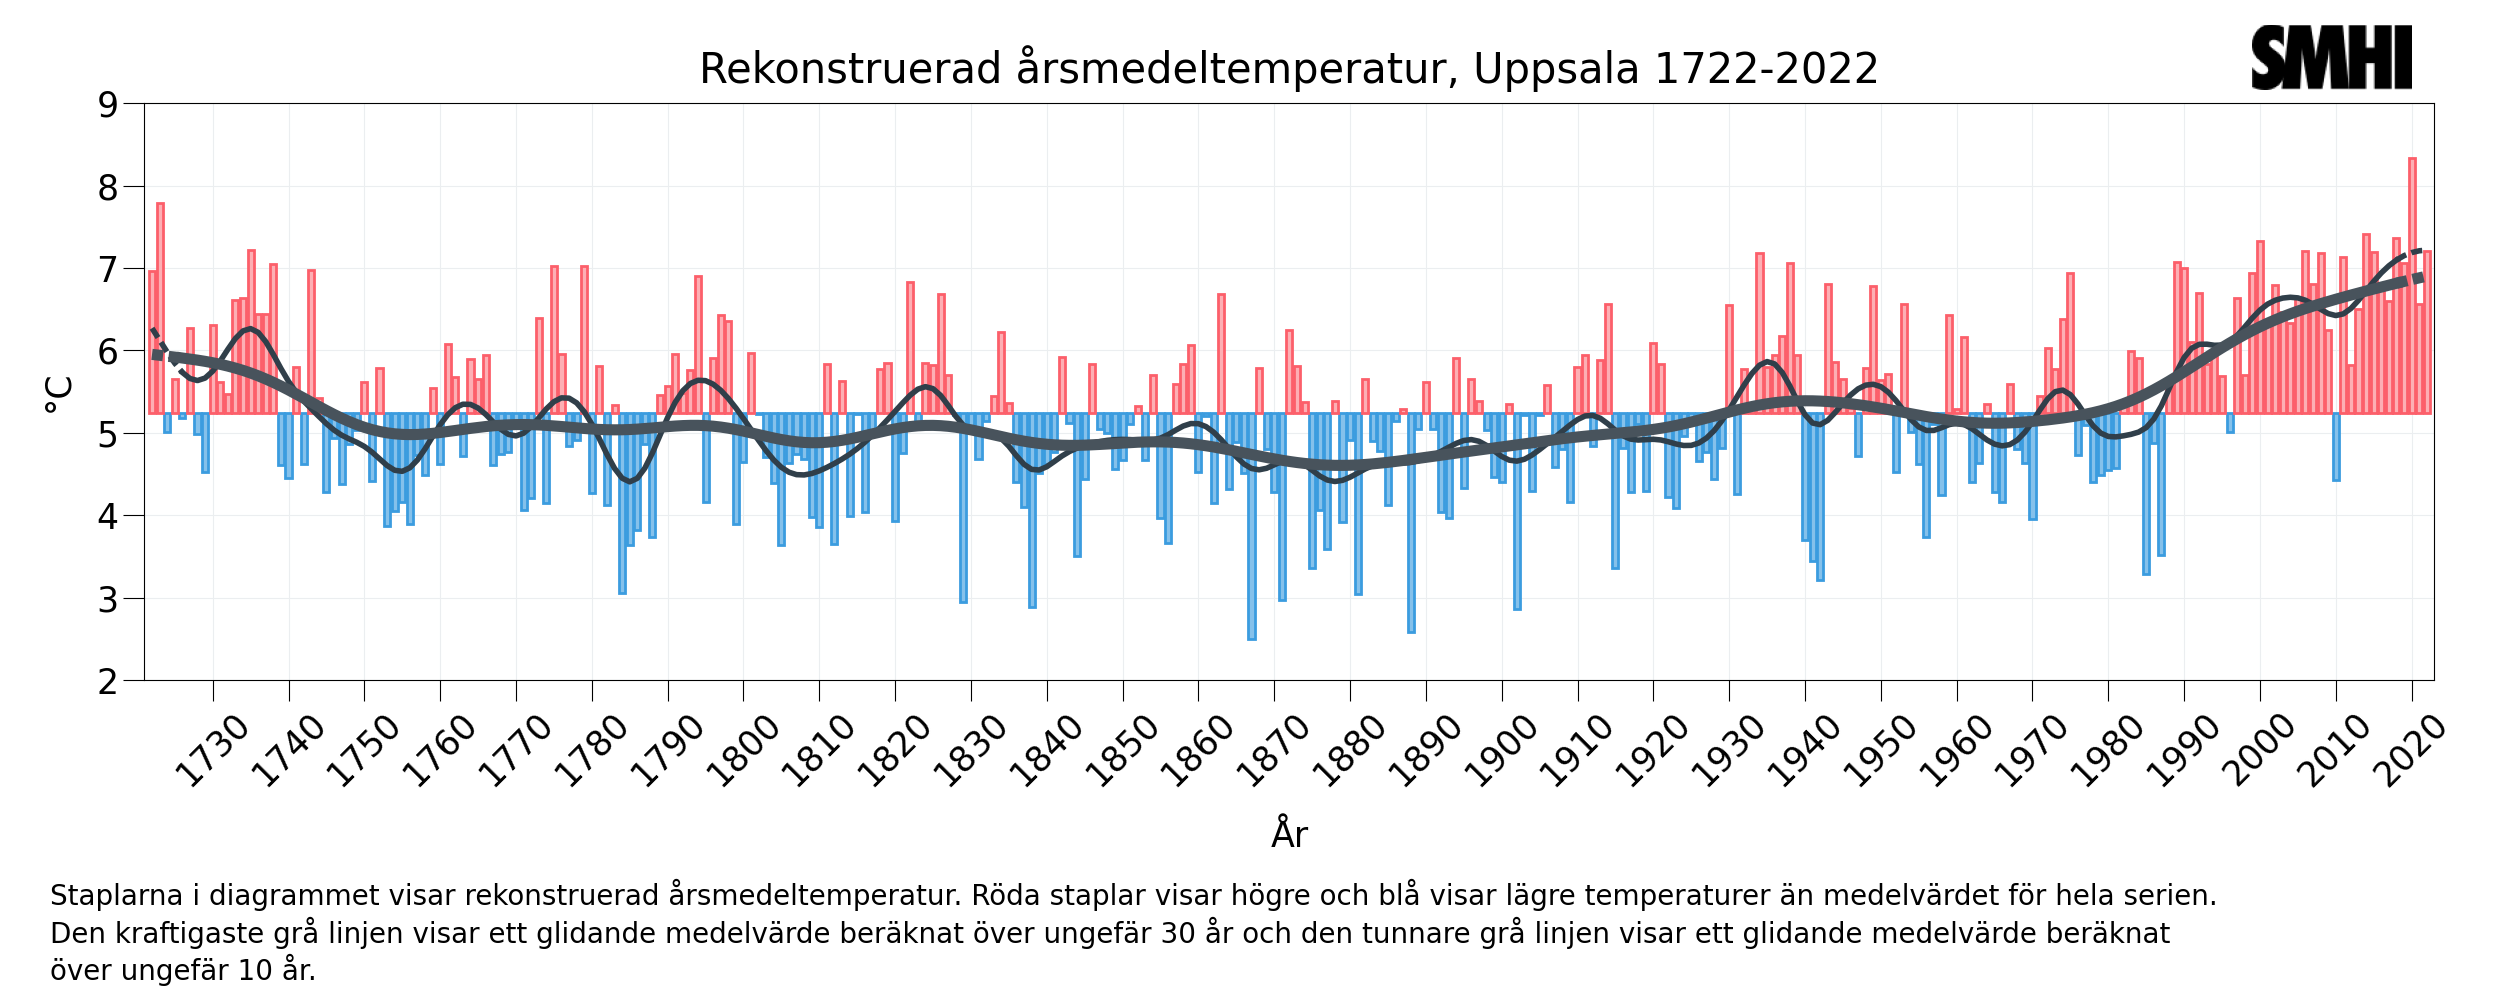
\includegraphics[width=\linewidth]{./data_trend.png}
      \caption{Yearly Trend}
      \label{fig:Trend}
    \end{figure}

    \section{Theoretical Background}
    State-space models are a powerful mathematical framework used to describe dynamic systems that evolve over time, making them especially useful in time series analysis, control systems, and signal processing. These models represent a system using two equations: a state equation, which captures the evolution of unobserved latent states, and an observation equation, which links these hidden states to observed data. Formally, a linear Gaussian state-space model is typically written as:
    \begin{gather}
      \mathbf{X}_t = \mathbf{A}_t \mathbf{X}_{t-1} + \mathbf{B}_t\mathbf{w}_t \\
      \mathbf{Y}_t = \mathbf{C}_t \mathbf{X}_t + \mathbf{D}_t\mathbf{v}_t
    \end{gather}
    where $\mathbf{X}_t$ is the state vector, $\mathbf{Y}_t$ is the observed vector and \(\mathbf{Y}_t \mid \mathbf{X}_t\) are independent for all $t$, $\mathbf{A}_t$ and $\mathbf{C}_t$ are system and observation matrices, and $\mathbf{w}_t , \mathbf{v}_t \sim \mathcal{N}(0, 1)$ and mutually independent Gaussian noise processes and $\mathbf{B}_t$ and $\mathbf{D}_t$ are the scale of the noises. This formulation allows for applying Bayesian inference techniques to estimate the hidden states and model parameters, making it a versatile tool for analyzing time series data. This could be done using MCMC to sample from the posterior distribution then it could be used to make predictions about the future values of the time series.

    One of the interesting facts about the state-space models is that we can build new models composing multiple state-space models together or even by making some assumptions the state-space model could be decomposed into simpler ones. In a classical point of view the state-space model has three components: the trend, the seasonal and the noise. The trend is the long-term movement in the data, the seasonal is the repetitive movement in the data and the noise is the random movement around a constant value. Where each of them are state-space models themselves and it is formally written as:
    \begin{gather}
      \mathbf{Y}_t = \mathbf{T}_t + \mathbf{S}_t + \mathbf{N}_t
    \end{gather}

    Where $\mathbf{T}_t$ is the trend component, $\mathbf{S}_t$ is the seasonal component and $\mathbf{N}_t$ is the noise component. The trend component could be modeled using a random walk or a local linear trend model.noise component could be modeled using a Gaussian noise or a t-distribution noise which could be iid or correlated during the time. I will discuss these three components in more details in the following sections. Another advantage of the classical time-series decomposition is its simplicity, interpretability and its capability to model each component separately.

    \subsection{Noise}
    The noise component is the random movement in the data which we assume to be stationary. It could be modeled using a Gaussian noise or a t-distribution noise which could be iid or correlated during the time. It could also be another state-space model itself. The noise component is important because it captures the random fluctuations in the data that cannot be explained by the trend or seasonal components. It could be modeled using Auto Regressive models which are members of the state-space model family are designed for stationary time-series. The AR(p) model is a linear regression model where the dependent variable is regressed on its own past values. The AR(p) model is written as:
  \begin{gather}
    \label{eq:ar}
    Z_t \mid Z_{t-1}, \cdots, Z_{t-p} \sim N_p(\beta \begin{pmatrix}
      1\\
      Z_{t-1}\\
      \vdots\\
      Z_{t-p}
    \end{pmatrix}, \sigma_N^2)
  \end{gather}
  where $Z_t$ is the observed variable, $Z_{t-1}, \cdots, Z_{t-p}$ are the past values of the observed variable, $\beta$ is the regression coefficient, and $\sigma^2_t$ is the variance of the noise. The AR(p) model is a special case of the state-space model where the state vector is the past values of the observed variable and the observation vector is the observed variable itself. The AR(p) model is a powerful model for stationary time-series data and it can be used to capture the autocorrelation in the data.

  \subsection{Trend}
  The trend component is the long-term movement in the data. It could be modeled using a random walk or a local linear trend model. The random walk model is a simple model where the current value of the observed variable is equal to the previous value plus a random noise. The local linear trend model is a more complex model where the current value of the observed variable is equal to the previous value plus a random noise and a trend component. The local linear trend model is written as:
  \begin{gather}
    \label{eq:trend}
    T_t \mid T_{t-1} \sim N(T_{t-1} + \mu_T, \sigma^2_T)\
  \end{gather}

  Which is a Gaussian random walk with drift \(\mu_T\). It distributed around a line with slope \(\mu_T\) and variance \(\sigma^2_T\). The local linear trend model is a powerful model for non-stationary time-series data and it can be used to capture the long-term trend in the data.

  \subsection{Seasons}
  Seasonal component is used to capture the repetitive behavioral pattern in the data. There are many state-space models that could be used for the modeling. For instance, the Fourier series which is a powerful tool to decompose signals into periodic components. However, in this report a more statistical approach is used. The idea is that the summation of data in one period should be a constant value or at least with some uncertainty around a constant value. Keeping this in mind the suggested model is given by:
  \begin{gather}
    \label{eq:seasonal}
    S_t \mid S_{t-1},\cdots, S_{t-p} \sim N(\sum_{i=1}^p S_{t-i}, \sigma^2_S)
  \end{gather}

  \section{Modeling}
  Now we create two models based on the classical model mentioned in the previous section. The first model is a simple AR(1) model where the observed variable is modeled using an AR(1) model. The second model is a more complex model where the observed variable is modeled using an AR(1) model with a seasonal component. The trend component is not included in the model as shown in \ref{fig:Trend} there is no clear linear trend on our data. The models are implemented using using PyMC to estimate the posterior using MCMC.And to reach a convergence we assumed \(\sigma_N = \sigma_S = \sigma\)

  \subsection{AR(1) Model}
  As we discussed how our data behaviour is unpredictable and noisy when we see the whole data from outside (See Figure \ref{fig:UppsalaTemperature}). The first suggested model is a simple AR(1) model where the observed variable is modeled using an AR(1) model with a Gaussian noise. Its architecture is shown in Fig. \ref{fig:ar1_model}  A visual inspection of the posterior mean and its performance on training set shown in Fig. \ref{fig:ar1_fit} shows that the model is able performing well on the values in the mid range while it needs improvement on extreme temperatures. Therefore, it is natural to observe in figure \ref{fig:ar1_ppc} that the model does not take into account the local maximum of the actual distribution. 

  \begin{figure}
    \begin{center}
      \includegraphics[width=0.95\linewidth]{../results/ar1/model_graph.png}
    \end{center}
    \caption{AR(1) Architecture}\label{fig:ar1_model}
  \end{figure}
  \begin{figure}
    \begin{center}
      \includegraphics[width=0.95\linewidth]{../results/ar1/stats/fit.png}
    \end{center}
    \caption{AR(1) Train data fit}\label{fig:ar1_fit}
  \end{figure}
  \begin{figure}
    \includegraphics[width=0.95\linewidth]{../results/ar1/stats/ppc.png}
    \caption{AR(1) PPC}\label{fig:ar1_ppc}
  \end{figure}

  \subsection{AR(1) with Seasonal Component}
  When we took a closer look into the data (See Fig. \ref{fig:UppsalaTemperatureSliced}) we noticed that the temperature behavior is not that much unpredictable and random as the temperature almost repeating itself every 12 months. Therefore, adding a seasonal component could be vital. The seasonal component model uses the formulation stated in Equation (\ref{eq:seasonal}) by setting $p=12$. The model is shown in Fig. \ref{fig:ar1_seasonal_model} and the performance on training set is shown in Fig. \ref{fig:ar1_seasonal_fit}. It can be seen that the model is able to capture the local maximum and minimum of the actual distribution which is also verified by the posterior predictive check shown in Fig. \ref{fig:ar1_seasonal_ppc}.
  \begin{figure}[ht!]
    \begin{center}
      \includegraphics[width=0.95\linewidth]{../results/ar1_s_1/model_graph.png}
    \end{center}
    \caption{AR(1) with Seasonal Component Architecture}\label{fig:ar1_seasonal_model}
  \end{figure}
  \begin{figure}
    \begin{center}
      \includegraphics[width=0.95\linewidth]{../results/ar1_s_1/stats/fit.png}
    \end{center}
    \caption{AR(1) + Seasonal Component}\label{fig:ar1_seasonal_fit}
  \end{figure}
  \begin{figure}
    \begin{center}
      \includegraphics[width=0.95\linewidth]{../results/ar1_s_1/stats/ppc.png}
          \end{center}
          \caption{AR(1) + Seasonal Component PPC}\label{fig:ar1_seasonal_ppc}
  \end{figure}
  \subsection{Model Comparison}
  The models are compared using  ELPD (Expected Log Pointwise Predictive Density) which is estimated using WAIC (Widely Applicable Information Criterion) \cite{waic} and \cite{EPLD}. The model with the higher ELPD and lower WAIC penalty is preferred. The results are shown in Table \ref{tab:model_comparison}. The $p_{waic}$ is the penalty term which is used to penalize the model complexity. It is natural to expect more complexity for the model with seasonal component while the final decisive metric is the $elpd_{waic}$ showing a dominance of the seasonal model over the AR(1) model.
  \begin{table}[ht!]
    \caption{Model Comparison}\label{tab:model_comparison}
    \begin{center}
      \begin{tabular}{lrrrrrrrrl}
      \toprule
       & rank & $elpd_{waic}$ & $p_{waic}$ \\
      \midrule
      ar1+seasonal & 0 & -6441.186400 & 1749.546770 \\
      ar1 & 1 & -9596.982600 & 828.905040 \\
      \bottomrule
      \end{tabular} 
    \end{center}
  \end{table}

  \subsection{Future Performance}
  The prediction of the future in time-series is not as simplicity as non time-series data. The future prediction depends on the previous step prediction or in terms of Bayesian modeling the prior of each step is the posterior of the previous step. Specifically, the last posterior of the model in training is used as the prior for the first step of the prediction. And this recursive process is repeated to cover our test dataset which 120 points. 
The Continuous Ranked Probability Score (CRPS) is used to evaluate the model performance on the test data. The CRPS is a scoring that measures the difference between the predicted and observed cumulative distribution functions. The CRPS is defined as:

\[
  CRPS(F, y) = \int_{-\infty}^{\infty} (F(x) - \mathbb{I}_{x\ge y})^2 dx
\]

By calculating the CRPS for each model, we can compare their performance on the test data. The results are shown in Table \ref{tab:crps}. The model with the lower CRPS is preferred. To visualize this the forecasts for shown in Figure \ref{fig:ar1_pred} and Figure \ref{fig:ar1_s_pred} where without seasonal component it flattens after a few steps while the chosen model maintains its shape. Which justifies the complexity of the seasonal model.

\begin{table}
  \caption{CRPS}\label{tab:crps}
  \begin{center}
    \begin{tabular}[c]{l|l}
      \hline
      \multicolumn{1}{c|}{\textbf{model}} & 
      \multicolumn{1}{c}{\textbf{crps}} \\
      \hline
      ar1 & 4.35 \\
      ar1+seasonality & 1.85 \\
      \hline
    \end{tabular}
  \end{center}
\end{table}
\begin{figure}
  \begin{center}
    \includegraphics[width=0.95\linewidth]{../results/ar1/stats/pred.png}
  \end{center}
  \caption{AR(1) Forecast}\label{fig:ar1_pred}
\end{figure}
\begin{figure}
  \begin{center}
    \includegraphics[width=0.95\linewidth]{../results/ar1_s_1/stats/pred.png}
  \end{center}
  \caption{AR(1) and Seasonal Component}\label{fig:ar1_s_pred}
\end{figure}
\subsection{Implementation}
The Python programming language was used for data exploration, modeling and visualization. Pandas Timeseries and DataFrame data structure where mainly used for data exploration together with Matplotlib for visualizaiton. For Bayesian modeling and MCMC PyMC \cite{pymc} is used. PyMC has a variety of functionalities for time-series modeling. It also has many examples of its use cases including time-series applications, survival analysis, and Bayesian regression. It could use JAX for faster computation and GPU support. The package is well documented and has a large community of users. Arviz \cite{arviz} is used for posterior analysis and visualization. It has a variety of functionalities for posterior predictive checks, model comparison, and diagnostics. It perfectly integrates with PyMC.

\section{Conclusion and Future Work}
During this report we explored the Uppsala temperature dataset and tried to find a suitable Bayesian model for it to be able to provide a forecast for the future. We used two models one an AR(1) and one which included an extra Seasonal component. We concluded that the model with the seasonal component is better in terms of ELPD and CRPS for historical and future respectively. It is worth noting how information about the seasonality in the model as an already known fact could improve the model performance. However, there are still some improvements that could be done. For instance, we assumed that the variance of seasonality has constant mean and is common with the noise component. It is suggested to use separate variances where for the seasonal component it should also change by the seasons. Another thing that could be improved is the trend component. In this report we did not include the trend component as there was no clear linear trend in the data. However, it is suggested to use a trend that could capture the non-linearity of the trend in our data.

  \  \bibliographystyle{IEEEtran}
    \bibliography{refs}

    \includepdf[pages=1-]{./codes.pdf}
\end{document}
